\chapter{Differentiation}
\section{The Derivative of a Real Function}
\begin{definition}
A function $f:[a,b]\to\RR$ is called \vocab{differentiable} at $x_0\in[a,b]$, if the limit of the function
\[ \phi(t)\coloneqq\frac{f(t)-f(x_0)}{t-x_0}, \quad a<t<b, t\neq x_0 \]
exists as $t\to x_0$. For this case, we write
\begin{equation}\label{eqn:derivative}
f^\prime(x_0)=\lim_{t\to x_0}\phi(t)=\lim_{t\to x_0}\frac{f(t)-f(x_0)}{t-x_0}.
\end{equation}
\end{definition}

The function $f$ is differentiable over $[a,b]$ if it is differentiable for each $x\in[a,b]$. It induces the function
\[ \dv{f}{x}=f^\prime:[a,b]\to\RR, \]
which is called the \vocab{derivative} of $f$.

\begin{theorem}\label{thrm:diff-cont}
If $f:[a,b]\to\RR$ is differentiable at $x_0\in[a,b]$, then it must be continuous at $x_0$.
\end{theorem}

\begin{proof}
As $t\to x$,
\[ f(t)-f(x)=\frac{f(t)-f(x)}{t-x}\cdot(t-x)\to f^\prime(x)\cdot0=0. \]
\end{proof}

\begin{remark}
The converse of this theorem is not true. It is easy to construct continuous functions which fail to be differentiable at isolated points.
\end{remark}

\begin{notation}
We use $C_1[a,b]$ to denote the set of differentiable functions over $[a,b]$ whose derivative is continuous. More generally, we use $C_k[a,b]$ to denote the set of functions whose $k$-th ordered derivative is continuous. In particular, $C_0[a,b]$ is the set of continuous functions over $[a,b]$.
\end{notation}

Later on when we talk about properties of differentiation such as the intermediate value theorems, we usually have the following requirement on the function:
\begin{quote}
$f$ is a continuous function on $[a,b]$ which is differentiable in $(a,b)$.
\end{quote}

\begin{theorem}[Differentiation rules]
Suppose $f,g:[a,b]\to\RR$ are differentiable at $x_0\in[a,b]$. Then $f\pm g$, $fg$ and $f/g$ (when $g(x_0)\neq0$) are differentiable at $x_0$. Moreover,
\begin{enumerate}[label=(\arabic*)]
\item $(f\pm g)^\prime(x_0)=f^\prime(x_0)\pm g^\prime(x_0)$;
\item $(fg)^\prime(x_0)=f^\prime(x_0)g(x_0)+f(x_0)g^\prime(x_0)$;
\item $\displaystyle\brac{\frac{f}{g}}^\prime(x_0)=\frac{f^\prime(x_0)g(x_0)-f(x_0)g^\prime(x_0)}{g(x_0)^2}$
\end{enumerate}
\end{theorem}

\begin{proof}
We take (2) as an example.

We calculate
\begin{align*}
\frac{f(x)g(x)-f(x_0)g(x_0)}{x-x_0}&=\frac{\brac{f(x)-f(x_0)}g(x)+f(x_0)\brac{g(x)-g(x_0)}}{x-x_0}\\
&=\frac{f(x)-f(x_0)}{x-x_0}\cdot g(x)+f(x_0)\cdot\frac{g(x)-g(x_0)}{x-x_0}\\
&\to f^\prime(x_0)g(x_0)+f(x_0)g^\prime(x_0)\text{ as }x\to x_0
\end{align*}
where we use $f$ and $g$ are differentiable at $x_0$ and Theorem \ref{thrm:diff-cont}.
\end{proof}

\begin{theorem}[Chain rule]
Let $f:[a,b]\to\RR$ be a real-valued function that is differentiable at $x_0\in[a,b]$. Let $g$ be a real-valued function defined on an interval that contains $f([a,b])$, and $g$ is differentiable at $f(x_0)$. Then the composition
\[ h(x)\coloneqq g\circ f(x)\coloneqq g\brac{f(x)}:[a,b]\to\RR \]
is differentiable at $x_0$ and the derivative at $x_0$ can be calculated as
\[ h^\prime(x_0)=g^\prime\brac{f(x_0)}f^\prime(x_0). \]
\end{theorem}

\begin{proof}
We know that
\[ f^\prime(x)=\lim_{t\to x}\frac{f(t)-f(x)}{t-x}, \]
so under the assumption that $t$ stays within the domain of $f$, $\frac{f(t)-f(x)}{t-x}$ should be a good approximation to $f^\prime(x)$.

To actually quantify this, let $u(t)=\frac{f(t)-f(x)}{t-x}-f^\prime(x)$.

Then the differentiability of $f$ tells us that $\lim_{t\to x}u(t)=0$.

Similarly, let $v(s)=\frac{g(s)-g(y)}{s-y}-g^\prime(y)$, then $\lim_{s\to y}v(s)=0$, as long as $s$ stays in the domain of $g$

What's nice here is that we can let $s=f(t)$, then by our assumption s always stays in the domain of g, so nothing fishy will happen

Ah I forgot a small detail here
Additionally we also need to define u(x)=0 and v(y)=0

Now let $h(t)=g(f(t))$, then $h$ is defined on $[a,b]$, and we deduce that
\[ h(t)-h(x)=(t-x)[f^\prime(x)+u(t)][g^\prime(y)+v(s)] \]

We then check that
\[ \lim_{t\to x}\frac{h(t)-h(x)}{t-x} = \lim_{t\to x}[f^\prime(x)+u(t)][g^\prime(y)+v(s)] = f^\prime(x)g^\prime(f(x)) \]
and we are done.
\end{proof}

%%%%%%%%%%%%%%%%%%%





\begin{example}
One of the best (worst?) family of pathological examples in calculus are functions of the form
\[ f(x)=x^p\sin\frac{1}{x}. \]
\begin{itemize}
\item For $p=1$, the function is continuous and differentiable everywhere other than $x=0$.
\item For $p=2$, the function is differentiable everywhere, but the derivative is discontinuous.
\end{itemize}

Other more advanced pathological results (just for fun):
\begin{itemize}
\item The graph for $y=\sin\dfrac{1}{x}$ on $(0,1]$, together with the interval $[-1,1]$ on the $y$-axis, is a connected closed set that is not path-connected.
\item For $0<p<1$, we obtain functions that are continuous and bounded, but the graphs are of infinite length (ps. I think that this is also true for $p=1$).
\end{itemize}
Regarding continuous but not differentiable functions, a more pathological example is the Weierstrass function, which is continuous everywhere over $\RR$ but differentiable nowhere.
\end{example}

\section{Mean Value Theorems}
\begin{definition}
Let $f$ be a real valued function defined over a metric space $X$. We say $f$ has a \vocab{local maximum} at $x_0\in X$ if $\exists\delta>0\suchthat\forall x\in B_\delta(x_0)$,
\[ f(x_0)\ge f(x). \]
Similarly, we say $f$ has \vocab{local minimum} at $x_0\in X$ if $\exists\delta>0\suchthat\forall x\in B_\delta(x_0)$,
\[ f(x_0)\le f(x). \]
\end{definition}

\begin{definition}
For a function $f:(a,b)\to\RR$, a point $x_0\in[a,b]$ is called a \vocab{critical point} if $f$ is not differentiable at $x_0$ or $f^\prime(x_0)=0$.
\end{definition}

\begin{theorem}
Assume $f$ is defined over $[a,b]$. If $f$ has a local maximum or local minimum at some $x_0\in(a,b)$, then $x_0$ is a critical point of $f$.
\end{theorem}

\begin{proof}
If $f$ is not differentiable at $x_0$, we are done. Assume now $f$ is differentiable at $x_0$ and $x_0$ is a local maximum.

Then $\exists\delta>0\suchthat\forall x\in B_\delta(x_0)$,
\[ f(x_0)\le f(x). \]
It follows
\[ \frac{f(x)-f(x_0)}{x-x_0}\begin{cases}
\ge0 & x_0-\delta<x<x+\delta\\
\le0 & x_0<x<x_0+\delta
\end{cases} \]
Further since $f^\prime(x_0)$ exists, there is
\[ f^\prime(x_0-)\ge0, \quad f^\prime(x_0+)\le0, \]
but $f^\prime(x_0-)=f^\prime(x_0+)=f^\prime(x_0)$. Hence $f^\prime(x_0)=0.$
\end{proof}

%We say that $x$ is a \vocab{stationary point} of $f$ if $f^\prime(x)=0$.

\begin{theorem}[Fermat's Theorem (Interior Extremum Theorem)]
If the differential exists, then by comparing the left and right limits it is easy to see that the differential for a local maximum/maximum can only be $0$.

To summarize in four words: Local extrema are stationary
\end{theorem}

There are three mean value theorems, from specific to general:
\begin{enumerate}
\item Rolle's Theorem
\item (Lagrange's) Mean Value Theorem
\item Generalised (Cauchy's) Mean Value Theorem
\end{enumerate}

\begin{theorem}[Rolle's Theorem]
If $f$ is continuous on $[a,b]$, differentiable in $(a,b)$ and $f(a)=f(b)$, then there exists $c\in(a,b)$ such that 
\[ f^\prime(c)=0. \]
\end{theorem}

\begin{proof}
Let $h(x)$ be a function defined on $[a,b]$ where $h(a)=h(b)$.

The idea is to show that $h$ has a local maximum/minimum, then by Fermat's Theorem this will then be the stationary point that we're trying to find.

First note that $h$ is continuous on $[a,b]$, so $h$ must have a maximum $M$ and a minimum $m$.

If $M$ and $m$ were both equal to $h(a)=h(b)$, then $h$ is just a constant function and so $h^\prime(x)=0$ everywhere.

Otherwise, $h$ has a maximum/minimum that is not $h(a)=h(b)$, so this extremal point lies in $(a,b)$.

In particular, this extremal point is also a local extremum.
Since $h$ is differentiable on $(a,b)$, by Fermat's theorem this extremum point is stationary, thus Rolle's Theorem is proven.
\end{proof}

\begin{theorem}[Mean Value Theorem]
If $f$ is continuous on $[a,b]$ and differentiable in $(a,b)$, then there exists $c\in(a,b)$ such that
\[ f^\prime(c)=\frac{f(b)-f(a)}{b-a}. \]
\end{theorem}

Exercise 2: Show that the Mean Value Theorem results directly from Rolle's Theorem (the other direction is trivial)
:
This isn't a very significant exercise because we're going to prove something more general

\begin{theorem}[Generalised Mean Value Theorem]
If $f$ and $g$ are continuous on $[a,b]$ and differentiable in $(a,b)$, then there exists $c\in(a,b)$ such that
\[ \frac{f^\prime(c)}{g^\prime(c)}=\frac{f(b)-f(a)}{g(b)-g(a)}. \]
\end{theorem}


Now we return to the proof of the generalized MVT

We set the function $h(t)=[f(b)-f(a)]g(t)-[g(b)-g(a)]f(t)$, then $h$ is continuous on $[a,b]$ and differentiable on $(a,b)$

Moreover, $h(a)=f(b)g(a)-f(a)g(b)=h(b)$, thus by Rolle's Theorem, there exists $c\in(a,b)$ such that $h^\prime(c)=0$, i.e. $[g(b)-g(a)]f^\prime(c)=[f(b)-f(a)]g^\prime(c)$

Corollary: If $f$ and $g$ are continuous on $[a,b]$ and differentiable in $(a,b)$, and $g^\prime(x)\neq0$ for all $x\in(a,b)$, then there exists \[ c\in(a,b) \suchthat f^\prime(c)/g^\prime(c)=[f(b)-f(a)]/[g(b)-g(a)] \]

This form of the generalized MVT will be used to prove the most beloved rule of high school students

exercises for the Mean Value Theorem

\begin{exercise}
Let $f$ and $g$ be continuous on $[a,b]$ and differentiable on $(a,b)$. If $f^\prime(x)=g^\prime(x)$, then $f(x)=g(x)+C$.
\end{exercise}

\begin{exercise}
Given that $f(x)=x^\alpha$ where $0<\alpha<1$. Prove that $f$ is uniformly continuous on $[0,+\infty)$.
\end{exercise}

\begin{exercise}[Olympiad level]
Let $f$ be a function continuous on $[0,1]$ and differentiable on $(0,1)$ where $f(0)=f(1)=0$. Prove that there exists $c\in(0,1)$ such that
\[ f(x)+f^\prime(x)=0. \]
\end{exercise}

\section{Darboux's Theorem}
Darboux's Theorem implies some sort of a 'intermediate value' property of derivatives that is similar to continuous functions

This is Theorem 5.12 in the book

Now first and foremost, the requirement for this statement is that f must be differentiable on [a,b], not just in (a,b)
Otherwise f'(a) and f'(b) may not make sense
:
One common theme in many of these problems is to construct auxiliary functions
Suppose that $f^\prime(a)<\lambda<f^\prime(b)$, then we construct the auxiliary function $g(x)=f(x)-\lambda x$
:
Then we only need to find a point $x\in(a,b)$ such that g'(x)=0
:
This means that we only need to find a local maximum/minimum, which by Fermat's Theorem has to be a stationary point as well
:
Now we look at the values of g near a and b
:
Exercise 1: Using the fact that $g^\prime(a)<0$ and $g^\prime(b)>0$, show that a and b are local maxima of $g$

Here we regard g as simply a function on $[a,b]$, so we only need to show that a,b are maximum and corresponding semi-open neighbourhoods $[a,a+\epsilon)$ and $(b-\epsilon,b]$
:
Let m=g'(a)<0 be the slope of the tangent at a
:
Then lim(h→0+)[g(a+h)-g(a)]/h=m<0
:
This means that there should exist $\delta>0$ such that for $0<h<\delta$, [g(a+h)-g(a)]/h<m/2<0
:
Now we can rewrite the above as
g(a+h)<g(a)+mh/2
:
Since m<0 and h>0, we obtain
$g(a+h)<g(a)$ for $0<h<\delta$
:
Thus this proves that x=a is a local maximum of g
A similar proof applies for x=b
:
Now since g is differentiable on [a,b], in particular it has to be continuous on [a,b]
:
Since [a,b] is compact, g([a,b]) is compact in R and thus g has both maximum and minimum values in [a,b]
:
Here we'll just focus on the minimum value
:
As we've shown, x=a is a 'strict' local maxima, in the sense that for any point $x\in(a,a+\epsilon)$, we actually have the strict inequality $g(x)<g(a)$
:
This means that x=a cannot be a local minimum
:
Similarly, x=b cannot be a local minimum, and therefore g achieves its minimum strictly inside (a,b)
:
Only then we can say that this local minimum is stationary
(This will not work otherwise; note that a and b are both local maxima but are not stationary points of g)
:
An interesting implication of Darboux's Theorem is that if f is differentiable on [a,b], then f' cannot have simple discontinuities (removable or jump discontinuities), simply because these discontinuities do not allow this 'intermediate value' property
:
However, we should recall certain pathological examples like f(x)=x² sin 1/x (f(0)=0)
Here f'(0)=lim(h→0)[x² sin 1/x-0]/x=0, but f'(x)=2x sin 1/x - cos 1/x, so f' is discontinuous at x=0

\section{L'Hopital's Rule}
\begin{theorem}[L'Hopital's Rule]
Assume $f,g$ are differentiable over $(a,b)$ with $g(x)\neq0$. If either
\begin{enumerate}[label=(\arabic*)]
\item $\lim_{x\to a}f(x)=0$ and $\lim_{x\to a}g(x)=0$; or
\item $\lim_{x\to a}|g(x)|=+\infty$,
\end{enumerate}
and
\[\lim_{x\to a}\frac{f^\prime(x)}{g^\prime(x)}=A\in[-\infty,+\infty]\]
assuming $g^\prime(x)\neq0$ over $(a,b)$, then
\[\lim_{x\to a}\frac{f(x)}{g(x)}=A.\]
\end{theorem}

\begin{proof}
Now the entire proof is quite tedious because there's actually eight main cases to think of
1. $\frac{0}{0}$ or $\frac{\infty}{\infty}$
2. a is normal or $a=-\infty$
3. A is normal or $A=\pm\infty$

We'll only prove the most basic one here:
0/0, a and A are normal
This is the case which will be required for Taylor series

First we define f(a)=g(a)=0, so that $f$ and $g$ are continuous at $x=a$

Now let $x\in(a,b)$, then $f$ and $g$ are continuous on $[a,x]$ and differentiable in $(a,x)$
:
Thus by Cauchy's Mean Value Theorem, there exists $\xi\in(a,x)$ such that
\[ \frac{f^\prime(\xi)}{g^\prime(\xi)}=\frac{f(x)-f(a)}{g(x)-g(a)}=\frac{f(x)}{g(x)} \]

For each $x$, we pick $\xi$ which satisfies the above, so that $\xi$ may be seen as a function of $x$ satisfying $a<\xi(x)<x$

Then by squeezing we have $\lim_{x\to a^+}\xi(x)=a$.

Since $\frac{f^\prime}{g^\prime}$ is continuous near $a$, the theorem regarding the limit of composite functions give
\[ \lim_{x\to a^+}\frac{f(x)}{g(x)} = \lim_{x\to a^+}\frac{f'(\xi)}{g'(\xi)} = \lim_{x\to a^+}\brac{\frac{f^\prime}{g^\prime}}(\xi(x)) = A \]

Now the same reasoning can be used for $b$ where we will use lim(x→b-) to replace all the $\lim_{x\to a^+}$, and $\xi$ will be a function which maps to $(x,b)$.
\end{proof}

\begin{example} \
\begin{itemize}
\item $\lim_{x\to0}\frac{1-\cos x}{x^2}=\frac{1}{2}$.
\item $\lim_{x\to+\infty}\frac{x^2}{e^{3x}}=0.$
\end{itemize}
\end{example}

\section{Taylor Expansion}
Consider a function $f:[a,b]\to\RR$. We first look at the mean value theorem from the viewpoint of approximations for $f(x)$ near a point $x=a$. We can regard the constant function
\[ f_0(x)=f(a) \]
as the \emph{zero order approximation} of $f(x)$. Then we ask if we can understand the remainder
\[ R_1(x)\coloneqq f(x)-f(a), \quad x\in[a,b] \]
for this approximation. For this, if we assume $f\in C_0[a,b]$ and $f^\prime$ exists over $(a,b)$, then the mean value theorem tells us that there exists some $a<\xi_x<x$ (here $\xi_x$ emphasises that $\xi$ depends on $x$) so that we can write $R_1$ as
\[ R_1(x)=f^\prime(\xi_x)(x-a). \]
This is saying that the derivative of $f$ can control the remainder $R_1(x)$ as an order 1 monomial.



%%%%%%%%%%%%%%%%

The main expression is as follows:
\begin{equation}
f(x)=f(a)+\frac{f^\prime(a)}{1!}(x-a)+\frac{f^{\prime\prime}(a)}{2!}(x-a)^2+\frac{f^{\prime\prime\prime}(a)}{3!}(x-a)^3+\cdots
\end{equation}

So for example we have the following (we've used the ones for $e^x$ and $\ln x$ for generating functions):
\begin{align*}
e^x &= 1+x+\frac{x^2}{2!}+\frac{x^3}{3!}+\cdots \\
\sin x &= x-\frac{x^3}{3!}+\frac{x^5}{5!}-\frac{x^7}{7!}+\cdots \\
\cos x &= 1-\frac{x^2}{2!}+\frac{x^4}{4!}-\frac{x^6}{6!}+\cdots \\
\ln(1+x) &= x-\frac{x^2}{2}+\frac{x^3}{3}-\frac{x^4}{4}+\cdots
\end{align*}

There's a lot of things to say about these equations, for example the one for $\ln(1+x)$ only works for $|x|<1$

Also, if you want the RHS of the expression to be an infinite power series, $f(x)$ has to be smooth (infinitely differentiable)

Even then, the power series may never converge to $f(x)$ at any interval, no matter how small
The most common example given here is $f(x)=e^\frac{-1}{x^2}$ (f(0)=0); the Taylor series for $f(x)$ is just $0$

Now sometimes we don't actually that nice of a property for f, we're often given that fact that $f$ is only finitely differentiable

Then we will have something along the lines of
\[ f(x)\approx f(a)+\frac{f^\prime(a)}{1!}(x-a)+\frac{f^{\prime\prime}(a)}{2!}(x-a)^2+\cdots+\frac{f^{(n)}(a)}{n!}(x-a)^n \]
where $f^{(n)}$ denotes the $n$-th differential.

There are two main forms of the statement regarding the error between the original function and the Taylor series estimate

The simpler form is what's known as the Peano form: Given that f is n times differentiable at $a$, then
\[ f(x)=f(a)+\frac{f^\prime(a)}{1!}(x-a)+\frac{f^{\prime\prime}(a)}{2!}(x-a)^2+\cdots+\frac{f^{(n)}(a)}{n!}(x-a)^n+o((x-a)^n) \]

To show this, we only need to show that we have the following limit:
\[ \lim_{x\to a}\frac{f(x)-{f(a)+\frac{f^\prime(a)}{1!}(x-a)+\frac{f^{\prime\prime}(a)}{2!}(x-a)^2+\cdots+\frac{f^{(n)}(a)}{n!}(x-a)^n}}{(x-a)^n}=0 \]

The basic idea is to use the L'Hopital Rule n times. The numerator becomes $f^{(n)}(x)-f^{(n)}(a)$ which approaches $0$, whereas the denominater is just $n!$, so the limit exists and is equal to $0$.

However, we need to verify all the necessary conditions for L'Hopital
:
Here the main problem is that we don't know if we have the 0/0 indeterminate at each step, so we'll need to check this for the k-th step where k=1,...,n

Fortunately, the k-th derivative of the numerator is
$f^{(k)}(x)-f^{(k)}(a)-(x-a)F_k(x)$ where $F_k$ is just a bunch of random stuff, so the numerator approaches $0$ as $x\to a$
The $k$-th derivative of the denominator is $n(n-1)\cdots(n-k+1)(x-a)^{n-k}$ so it also approaches $0$, and we're done

The other form is actually a family of similar statements which gives more precise values for the error
The Peano form has a fundamental obstacle when used in approximation, we don't have any control on the size of the final term other than its asymptotic behaviour
:
We'll be talking about the one given in the book, known as the Lagrange form:
:
Given that f is n times differentiable on $(a,b)$ such that $f^{(n-1)}$ is continuous on $[a,b]$, then
\[ f(x)=f(a)+\frac{f^\prime(a)}{1!}(x-a)+\frac{f^{\prime\prime}(a)}{2!}(x-a)^2+\cdots+\frac{f^{(n-1)}(a)}{(n-1)!}(x-a)^(n-1)+\frac{f^{(n)}(\xi)}{n!}(x-a)^n \]

Just like in L'Hopital, we intuitively think of $(a,b)$ as just a very small interval at the right hand side of x=a
:
Here we are giving up on the second final term of Peano by combining it with the infinitesimal (small o) term to give an accurate description of the error

For the proof of this one we'll be using Cauchy's MVT

Fix any $x\in(a,b)$, then we construct the functions
\[ F(t)=f(x)-\brac{f(t)+\frac{f^\prime(t)}{1!}(x-t)+\frac{f^{\prime\prime}(t)}{2!}(x-t)^2+\cdots+\frac{f^{(n-1)}(t)}{(n-1)!}(x-t)^{n-1}} \]
\[ G(t)=(x-t)^n \]

We calculate $F^\prime(t)$ as follows:
\[ -[f^\prime(t)+\frac{f^{\prime\prime}(t)}{1!}-f^\prime(t)+\frac{f^{\prime\prime\prime}(t)}{2!}-\frac{f^{\prime\prime}(t)}{1!}+\cdots+\frac{f^{(n)}(t)}{(n-1)!}(x-t)^{n-1}-\frac{f^{(n-1)}(t)}{(n-2)!}(x-t)^{n-2}]=-\frac{f^{(n)}(t)}{(n-1)!}(x-t)^{n-1} \]

$G^\prime(t)=-n(x-t)^{n-1}$, so we have
\[ \frac{F^\prime(t)}{G^\prime(t)}=\frac{f^{(n)}(t)}{n!} \]

The main reason for why we come up with the strange-looking $F$ and $G$ is that we specifically swap out $a$ for $t$ so that $F(x)=G(x)=0$, in hopes of getting rid of $x$:

We apply Cauchy's MVT to $F$ and $G$ on $[a,x]$, so that we obtain $\xi\in(a,x)$ satisfying
\[ \frac{F^\prime(\xi)}{G^\prime(\xi)}=\frac{F(x)-F(a)}{G(x)-G(a)}=\frac{F(a)}{G(a)}. \]
Thus the Lagrange form of the remainder is given by 
\[ F(a)=\frac{f^{(n)}(\xi)}{n!}G(a). \]

Theorem 5.19 is important, so do go through that proof as an exercise

\chapter{Riemann--Stieltjes Integral}
\section{Definition of Riemann--Stieltjes Integral}
Assume $[a,b]$ is a closed interval in $\RR$. By a \vocab{partition} $P$, we mean a finite set of points $x_0,x_1,\dots,x_n$ where
\[ a=x_0\le x_1\le\cdots\le x_{n-1}\le x_n=b. \]
Assume $f$ is a bounded real-valued function over $[a,b]$ and $\alpha$ is an increasing function over $[a,b]$. Denote by
\[ M_i=\sup_{[x_{i-1},x_i]}f(x), \quad m_i=\inf_{[x_{i-1},x_i]}f(x) \]
and by
\[ \Delta\alpha_i=\alpha(x_i)-\alpha(x_{i-1}). \]
Define the \vocab{upper sum} of $f$ with respect to the partition $P$ and $\alpha$ as
\[ U(f,\alpha;P)=\sum_{i=1}^n M_i \Delta \alpha_i \]
and the \vocab{lower sum} of $f$ with respect to the partition $P$ and $\alpha$ as
\[ L(f,\alpha;P)=\sum_{i=1}^n m_i \Delta \alpha_i. \]
Define the upper Riemann--Stieltjes integral as
\[ \upperint_a^bf(x)\dd{\alpha(x)}\coloneqq\inf_P U(f,\alpha;P) \]
and the lower Riemann--Stieltjes integral as
\[ \lowerint_a^bf(x)\dd{\alpha(x)}\coloneqq\sup_P L(f,\alpha;P). \]
It is easy to see from definition that
\[ \lowerint_a^bf(x)\dd{\alpha(x)}\le\upperint_a^bf(x)\dd{\alpha(x)}. \]

\begin{definition}
A function $f$ is \vocab{Riemann--Stieltjes integrable} with respect to $\alpha$ over $[a,b]$, if
\[ \lowerint_a^bf(x)\dd{\alpha(x)}=\upperint_a^bf(x)\dd{\alpha(x)}. \]
\end{definition}

\begin{notation}
We use $\displaystyle\int_a^bf(x)\dd{\alpha(x)}$ to denote the common value, and call it the Riemann--Stieltjes of $f$ with respect to $\alpha$ over $[a,b]$.
\end{notation}

\begin{notation}
We use the notation $R_\alpha[a,b]$ to denote the set of Riemann--Stieljes integrable functions with respect to $\alpha$ over $[a,b]$.
\end{notation}

In particular, when $\alpha(x)=x$, we call the corresponding Riemann--Stieljes integration the \vocab{Riemann integration}, and use $R[a,b]$ to denote the set of Riemann integrable functions.

\begin{definition}
The partition $P^\prime$ is a \vocab{refinement} of $P$ if $P^\prime\supset P$. Given two partitions $P_1$ and $P_2$, we say that $P^\prime$ is their \vocab{common refinement} if $P^\prime=P_1\cup P_2$.
\end{definition}

Intuitively, a refinement will give a better estimation than the original partition, so the upper and lower sums of a refinement should be more restrictive.

\begin{proposition}
If $P^\prime$ is a refinement of $P$, then
\[ L(f,\alpha;P)\le L(f,\alpha;P^\prime) \]
and
\[ U(f,\alpha;P^\prime)\le U(f,\alpha;P). \]
\end{proposition}

\begin{proof}
Suppose that
\[ P: a\le x_0\le x_1\le ...\le x_n=b \]
and
\[ P^\prime: a\le y_0\le y_1\le ...\le y_m=b. \]
Then there exists a strictly increasing sequence of indices $j_0=0,j_1,\dots,j_n=m$ such that $y_{j_k}=x_k$.

Now consider each closed interval $[x_{i-1},x_i]$
%(From my definition of partitions, points may be equal; though if $x_{i-1}=x_i$, then both the set of points $\{x_{i-1},x_i\}$ in $P$ and $\{y_{j_{i-1}}, y_{j_{i-1}_1},\dots,y_{j_i}\}$ in $P^\prime$ will contribute nothing towards the upper and lower sums of P and $P^\prime$ respectively)

Focusing on the upper sum, we have
\[ \sup_{[x_{i-1},x_i]} f \ge \sup_{[y_{k-1},y_k]} f \]
for $k=j_{i-1}+1,\dots,j_i$. 
This is because $[y_{k-1},y_k]$ is contained in $[x_{i-1},x_i]$

\begin{figure}[H]
    \centering
    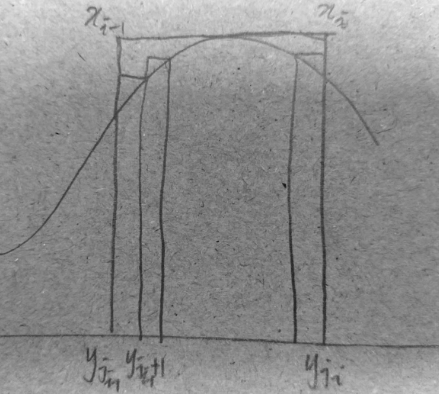
\includegraphics[width=0.5\linewidth]{images/RSintegral-partitions.png}
    \caption{Partitions}
\end{figure}

Continuing from
\[ \sup_{[x_{i-1},x_i]} f \ge \sup_{[y_{k-1},y_k]} f, \]
We then multiply by $\alpha(y_k)-\alpha(y_{k-1})$ on both sides and then take the sum from $k=j_{i-1}+1$ to $k=j_i$
:
The RHS corresponds to the (weighted) sum of the thin rectangles that you see in the above picture
:
The LHS is actually a telescoping sum, and the sum would be
\[ (\sup_{[x_{i-1},x_i]} f) \cdot [\alpha(y_{j_i})-\alpha(y_{j_{i-1}})] = (\sup_{[x_{i-1},x_i]} f) \cdot [\alpha(x_i)-\alpha(x_{i-1})] \]
Finally, we take the sum from $i=1$ to $i=n$ of the above inequality
LHS $\ge$ RHS (sorry I don't know of a better way to put it)
We then obtain $U(P,f,\alpha)\ge U(P^\prime,f,\alpha)$

(On the LHS we're collecting all the rectangles for the upper sum wrt $P$, but on the RHS we're collecting up collections of upper rectangles to obtain the entire collective of upper rectangles for the upper sum wrt $P^\prime$)
:
Lower sum is similar
:
Now, a lemma used to prove 6.5
Given any two partitions $P_1$ and $P_2$, we have
\[ L(P_1,f,\alpha)\le U(P_2,f,\alpha) \]
So a lower sum will always be no larger than any other upper sum
:
So this includes the cases where we have the most refined of $P_1$'s and $P_2$'s, with no information regarding the partition points whatsoever
To be honest, the result seems to be both intuitive and unclear at the same time

The key here is to use common refinements as a link for both sums
The idea is stated in the proof of 6.5 and I don't think I need to elaborate further

What's nice here is that now we have two completely independent partitions $P_1$ and $P_2$, so by fixing one partition, say $P_2$, and taking the 'limit' over the other (here we take the supremum over all possible $P_1$) we then obtain an inequality between a Darboux integral and a Darboux sum (here it's the lower integral and an upper sum)

Since the Darboux integral is just a number, we can then safely take the 'limit' over the other partition to obtain the inequality in 6.5
\end{proof}

\begin{proposition}
\[ \lowerint_a^bf\dd{\alpha}=\upperint_a^bf\dd{\alpha}. \]
\end{proposition}

\begin{proof}

\end{proof}

Now we move on to integrability conditions for $f$. The first one looks a lot like the $\epsilon-N$ or $\epsilon-\delta$ definition of limits:

\begin{theorem}
$f\in R_\alpha[a,b]$ if and only if for each $\epsilon>0$, there exists some partition $P$ such that
\[ U(f,\alpha;P)-L(f,\alpha;P)<\epsilon. \]
\end{theorem}
%%%%%%%%%%%%%%%%%%%%

\begin{proof} \

($\implies$) Assume $f\in R_\alpha[a,b]$. By definition,
\[ \inf_PU(f,\alpha;P)=\int_a^bf\dd{\alpha}=\sup_PL(f,\alpha;P). \]
For every $\epsilon>0$, 

($\impliedby$) 
\end{proof}



%%%%%%%%%%%%%%%%%%%%%%%%%
% Darboux sums, Darboux integrals

\begin{example}[Dirichlet function]
The Dirichlet function is given by
\[ f(x)=\begin{cases}
1 & x\in\QQ \\
0 & x\notin\QQ
\end{cases} \]
We try to calculate the two on the interval $[0,1]$.

The Dirichlet function is pathological because for each subinterval $[x_{i-1},x_i]$, the supremum is always $1$ and the infimum is always $0$.

So no matter what partition we use, $U(f,P)$ is always $1$ whereas $L(f,P)$ is always $0$. This means that $U(f)=1$ and $L(f)=0$, so there are two different values for ``the integral of $f$''.

This is like the case where we try to find the limit of the Dirichlet function where $x$ is approaching any given real number $r$, there exists two sequences approaching $r$ whose image approaches two different values.
\end{example}

Now, a very important and fun case about the more general RS-integral, which we'll discuss next week (do try the exercise yourself first)

\begin{exercise}
The Heaviside step function $H$ is a real-valued function defined by the following:
\[ H(x)=\begin{cases}
0 & x<0 \\
1 & x\ge0
\end{cases} \]
For the purpose of this question we assume the convention $\infty\cdot0=0$.
\begin{enumerate}[label=(\alph*)]
\item Let $f$ be a real-valued function over $\RR$. Show that $f\in\RR_H [a,b]$ if and only if $f$ is continuous at $0$, and find the RS-integral $\int_{-\infty}^\infty f\dd{H}$.
\item Suppose that the definition for $H$ is changed for $x=0$, say $H(0)=\frac{1}{2}$. Show that the above result still holds.
\item Examine the RS-integral of $f$ over $\RR\setminus\{0\}$ wrt $H$, where $f$ is a real-valued function over $\RR\setminus\{0\}$ such that $\lim_{x\to0}f(x)=\infty$ or $-\infty$.
\end{enumerate}
(You may read up on more information regarding the Heaviside function, and the (in)famous Dirac delta function)
\end{exercise}




Now we've been talking a lot about upper and lower sums because they're arguably the simplest way to define integrals, in the sense that there's not a whole lot of things that we could go wrong here
By considering only upper and lower bound, we're essentially picking the most conservative route possible

It would be nice if we could just pick like one random point within each interval and consequently calculate the Riemann(-Stieltjes) sums

This method, of course, fails to be well defined for pathological functions like the Dirichlet function
On the other hand, by using upper and lower sums, we could give a persuasive explanation as to why the Dirichlet function is not Riemann integrable

However, instead of throwing this idea away, there's actually a way for us to make this into a strict definition

When we were talking about the sequential definition for limits of functions, we noted that there are certain scenarios where the limit cannot exist because there may be two distinct sequences may give different limit
Based on this observation, we then gave a reasonable condition as follows:
"$\lim_{x\to a} f(x)$ exists and is equal to $L$ if and only if for all sequences $x_n$ converging but not containing a, $f(x_n)$ converges to $L$"

Well here, it's actually the same kind of scenario
Given any partition $P$, we consider the Riemann sum $\sum f(\xi_i)\Delta x_i$ where $\xi_i$ is any point where $x_{i-1}\le\xi_i\le x_i$

For the Dirichlet function over $[0,1]$, given any partition P (here we may assume that the partition points are distinct), we will always be able to specifically pick $\xi_i,\eta_i\in[x_{i-1},x_i]$ such that $\xi_i$ is rational but $\eta_i$ is irrational

Then $\sum f(\xi_i)\Delta x_i=1$ but $\sum f(\eta_i)\Delta x_i=0$

Now be very mindful that this alone cannot be evidence that f is non-integrable
The key is that this somehow occured for all partitions P, no matter how refined they are; for every single partition P, there exists two sets of 'representing points' $\xi_i,\eta_i$ such that the two Riemann sums are constantly far apart (1 and 0 in this case)

Let $\epsilon_0=1$, then this ultimately translates to the following:
The Dirichlet function cannot be Riemann integrable because
There exists some $\epsilon_0>0$, such that for any given partition $P$, there exists two sets of representing points $\xi_i,\eta_i$ such that their corresponding Riemann sums satisfy that
\[ |\sum f(\xi_i)\Delta x_i - \sum f(\eta_i)\Delta x_i|\ge\epsilon_0. \]

Now if we always pick the representatives such that $\xi_i>\eta_i$ then we can neglect the absolute value

So now, let's take the converse
A function $f$ is said to be RS-integrable if
For every $\epsilon>0$,
There exists a partition P, such that
For any two sets of representing points $\xi_i,\eta_i$,
Their corresponding Riemann sums satisfy that
\[ \sum[f(\xi_i)-f(\eta_i)]\Delta x_i<\epsilon \]
(The last one should be $\Delta \alpha_i$ for RS-integrals, not $\Delta x_i$)

Unfortunately this is still not quite the correct definition according to Apostol, but we're pretty close
The problem with this definition is that it is too weak if we're considering general $\alpha$ of bounded variation; if we were only talking about monotonically increasing $\alpha$ then this will actually be an equivalent definition

The official definition for the RS-integral wrt $\alpha$ of bounded variation is as follows:
\begin{definition}
For every $\epsilon>0$, there exists a partition $P$, such that
[For any refinement $P^\prime$ of P, and]
For any two sets of representing points $\xi_i,\eta_i$ [of $P^\prime$], their corresponding Riemann sums satisfy that
\[ \sum[f(\xi_i)-f(\eta_i)]\Delta x_i<\epsilon. \]
\end{definition}

Now this definition is what mathematicians would refer to as a 'Cauchy' definition, since it defines a notion by comparing a pair of arbitrary values that are similar to one another, and if they agree in some sense then we say that that something satisfies some property.

The integral is then obtained as follows: If $f$ were to satisfy the above Cauchy definition, then we may pick an arbitrary sequence of refinements
\[ P_1 \subset P_2 \subset P_3 \subset ...; \]
and for each partition we pick a set of representatives to obtain a sequence RS-sum
$I_1, I_2, I_3, ...$
:
This sequence will be a Cauchy sequence of real numbers, and so will converge to a specific value $I$ which we consider to be RS-integral of f
:
Now the reason why Apostol needed to strengthen the definition is that, otherwise this value $I$ may not be unique
:
So if you look at the statement you see in 6.7(b)(c), then they correspond to the Cauchy definition and the 'value-based' definition respectively
For monotonically increasing $\alpha$, it is much easier to discuss them using upper and lower sums
So your exercise today will be to read the statements and proofs in Theorem 6.7

\begin{theorem}
$f\in R_\alpha[a,b]$, $m\le f\le M$, and $\phi$ is uniformly continuous on $[m,M]$, then
\[ \phi\circ f\in R_\alpha[a,b]. \]
\end{theorem}

\begin{proof}
Choose $\epsilon>0$. Since $\phi$ is uniformly continuous on $[m,M]$, there exists $\delta>0$ such that $\delta<\epsilon$ and $|\phi(s)-\phi(t)|$
\end{proof}

\section{Properties of the Integral}
\begin{theorem} \
\begin{enumerate}[label=(\arabic*)]
\item If $f_1,f_2\in R_\alpha[a,b]$, then 
\[ f_1+f_2\in R_\alpha[a,b]; \]
$cf\in R_\alpha[a,b]$ for every $c\in\RR$, and
\[ \int_a^b(f_1+f_2)\dd{\alpha}=\int_a^bf_1\dd{\alpha}+\int_a^bf_2\dd{\alpha}, \]
\[ \int_a^b(cf)\dd{\alpha}=c\int_a^bf\dd{\alpha}. \]

\item If $f_1,f_2\in R_\alpha[a,b]$ and $f_1\le f_2$, then
\[ \int_a^bf_1\dd{\alpha}\le\int_a^bf_2\dd{\alpha}. \]

\item If $f\in R_\alpha[a,b]$ and $c\in[a,b]$, then $f\in R_\alpha[a,c]$ and $f\in R_\alpha[c,b]$, and
\[ \int_a^bf\dd{\alpha}=\int_a^c\dd{\alpha}+\int_c^b\dd{\alpha}. \]

\item If $f\in R_\alpha[a,b]$ and $|f|\le M$, then
\[ \absolute{\int_a^bf\dd{\alpha}}\le M\sqbrac{\alpha(b)-\alpha(a)}. \]

\item If $f\in R_{\alpha_1}[a,b]$ and $f\in R_{\alpha_2}[a,b]$, then $f\in R_{\alpha_1+\alpha_2}[a,b]$ and
\[ \int_a^bf\dd{(\alpha_1+\alpha_2)}=\int_a^bf\dd{\alpha_1}+\int_a^bf\dd{\alpha_2}; \]
if $f\in R_\alpha[a,b]$ and $c$ is a positive constant, then $f\in R_{c\alpha}[a,b]$ and
\[ \int_a^bf\dd{(c\alpha)}=c\int_a^bf\dd{\alpha}. \]

\item If $f\in R_\alpha[a,b]$ and $g\in R_\alpha[a,b]$, then $fg\in R_\alpha[a,b]$.
\end{enumerate}
\end{theorem}

\begin{proof} \
\begin{enumerate}[label=(\arabic*)]
\item If $f=f_1+f_2$ and $P$ is any partition of $[a,b]$, we have
\begin{align*}
L(f_1,\alpha;P)+L(f_2,\alpha;P)&\le L(f,\alpha;P)\\
&\le U(f,\alpha;P)\\
&\le U(f_1,\alpha;P)+U(f_2,\alpha;P).
\end{align*}

If $f_1\in R_\alpha[a,b]$ and $f_2\in R_\alpha[a,b]$, let $\epsilon>0$ be given. There are partitions $P_1$ and $P_2$ such that


\item 
\item 
\item 
\item 
\item 
\end{enumerate}
\end{proof}

\begin{theorem}[Triangle inequality]
$f\in R_\alpha[a,b]$, then $|f|\in R_\alpha[a,b]$,
\[ \absolute{\int_a^bf\dd{\alpha}}\le\int_a^b|f|\dd{\alpha}. \]
\end{theorem}

\begin{proof}

\end{proof}

6.14 6.15
Heaviside step function

6.16 corollary
for intinite sum, need $\sum c_n$ to converge
(23) comparison test

6.17 integration by substitution
\begin{theorem}
$\alpha$ increasing, $\alpha^\prime\in R[a,b]$, $f$ bounded on $[a,b]$, then
\[ f\in R_\alpha[a,b]\iff f\alpha^\prime\in R[a,b]. \]
\end{theorem}

6.19 change of variables

\section{Fundamental Theorem of Calculus}
6.20 6.21

\begin{theorem}

\end{theorem}

6.22 integration by parts